%!TEX root = ../crimson_throne_book_main.tex
% 2015-10-03
After a hearty meal Glorio takes his guest into his greenhouse garden,\hyperref[fig:Arkona-palace-garden-with-elephant-statue-563929835]{ which is filled with jungle plants, tropical birds and a refreshing fountain. The most surprising feature in the chamber is a life-sized statue of an elephant, its tusks and trunk raised high. } It takes Sjo a few seconds to realize this animal is not real, but made of stone. Glorio approaches the elephants and presses a hidden button somewhere, making the ground between the statue's giant feet shift aside to reveal a set of stairs. \\

\begin{figure}[h]
	\centering
	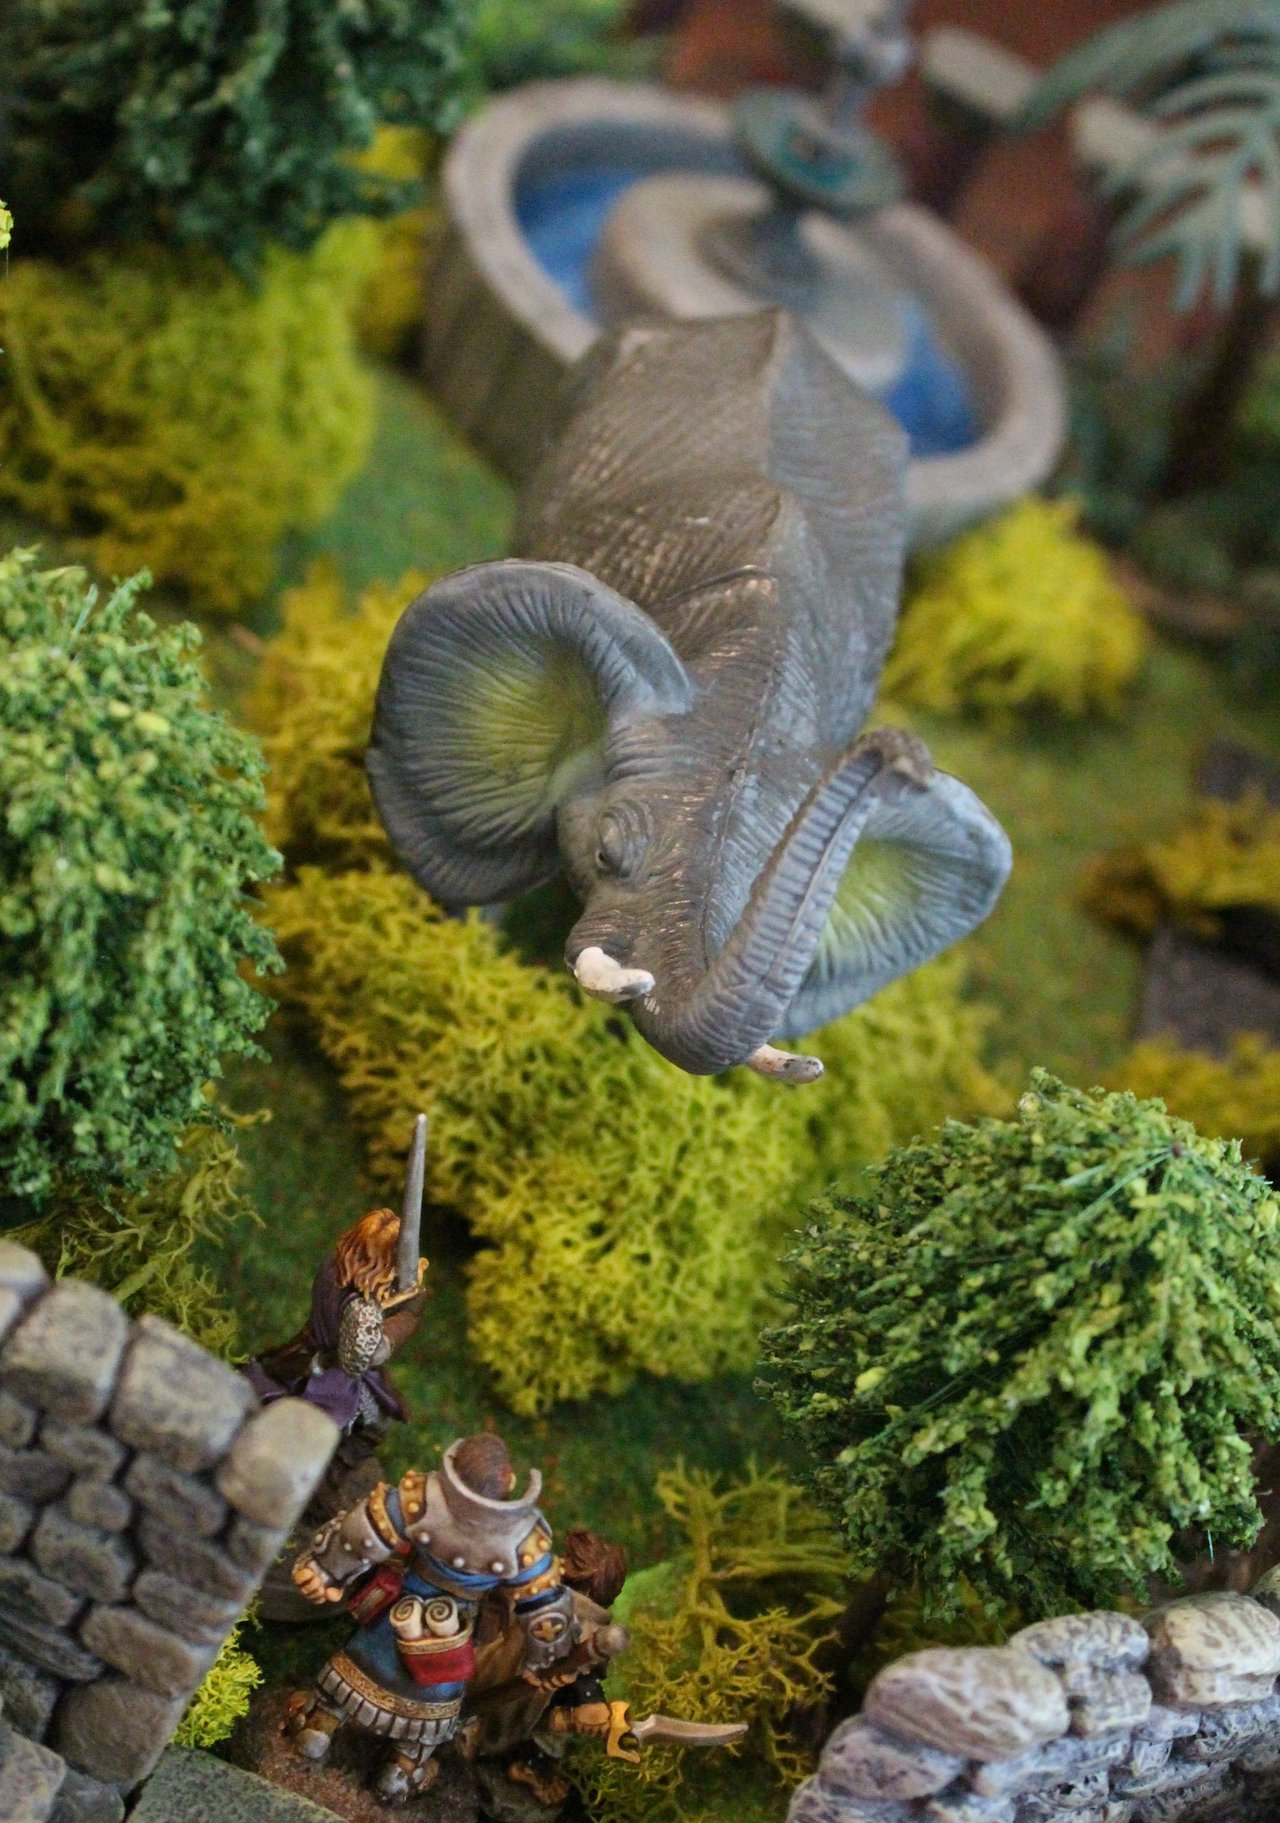
\includegraphics[width=0.39\textwidth]{images/Arkona-palace-garden-with-elephant-statue-563929835.jpg}
	\caption{Arkona palace garden with elephant statue}
	\label{fig:Arkona-palace-garden-with-elephant-statue-563929835}
\end{figure}

The companions follow their host down into a vast cavern under the palace. The air is cool, humid and smells of salt. Staring down from the upper ledge, Balian sees a number of rope bridges descending from ledge to ledge until they reach a small quay below. So this is how the Arkona's manage to keep their pantries full, a secret pier inside a sea cave; the perfect place to smuggle goods in or out unseen. The upper rim is overgrown with colored fungi and leads past a solemn tree that moves as our friends approach. Quint notices that Glorio waves his hand, making the tree lean back and stop swaying. Crossing a first rope bridge takes the companions to a ledge with a door in the wall, which Glorio completely ignores. He continues to a second, smaller ledge which has nothing but a natural wall. Sjo spots double doors on the bottom level, facing the pier in the sloshing pool of sea water, and wonders about them. Glorio says that they hold his family's private shrine to Chamidu, their Vudran patron deity.\\

Puk already wants to take the third and last rope bridge down, but Glorio stops him. The nobleman pushes against the blank cavern wall, opening a secret door into a hidden tunnel. "We're going this way, Puk." After 20 yards the tunnel makes a sharp turn to the left, leading up to a sturdy bronze door. The face of the bronze entryway and the arch around it are carved with motives of tigers chasing tigers in endless circles. Glorio seems to shrink back in sight of the entry to the labyrinth. "This is the place", he breathes. "This is a far as I go. I wish you the best of luck. I'll eagerly wait for your return, so hurry back."\\

Puk touches the bronze door and it swings open easily. The small entry room has an exit in the opposite wall. Once all the companions are inside, the bronze door behind them swings shut. Balian and Puk look for traps and when they find none, they open the other door, discovering a second door immediately behind it. After opening that one as well,\hyperref[fig:Vivified-labyrinth-entrance-563930398]{ the party walks into a room with two alcoves on either side and a statue at the far end. } Puk discovers two obvious pressure plates in both alcoves, while Quint studies the statue. It is the same man he saw on the painting in the lounge earlier, Eduardo Arkona, the builder of this labyrinth. The statue is dressed in long Vudran robes, has a shawl draped elegantly around its head and stretches out its hands to the sides. A familiar saying on the pedestal reads: "Balance in all things". Once Balian and Puk have established that the pressure plates do not trigger any traps, Quint figures out that both plates have to be pressed with a similar weight to trigger the mechanism. He steps and the left plate and motion for Balian to mount the other one. As soon as the ranger does so, the door slams shut and the companions feel the room turning. Puk estimates they have made a quarter turn before they stop and the door swings open again, revealing stairs going up to yet another door. \\

\begin{figure}[h]
	\centering
	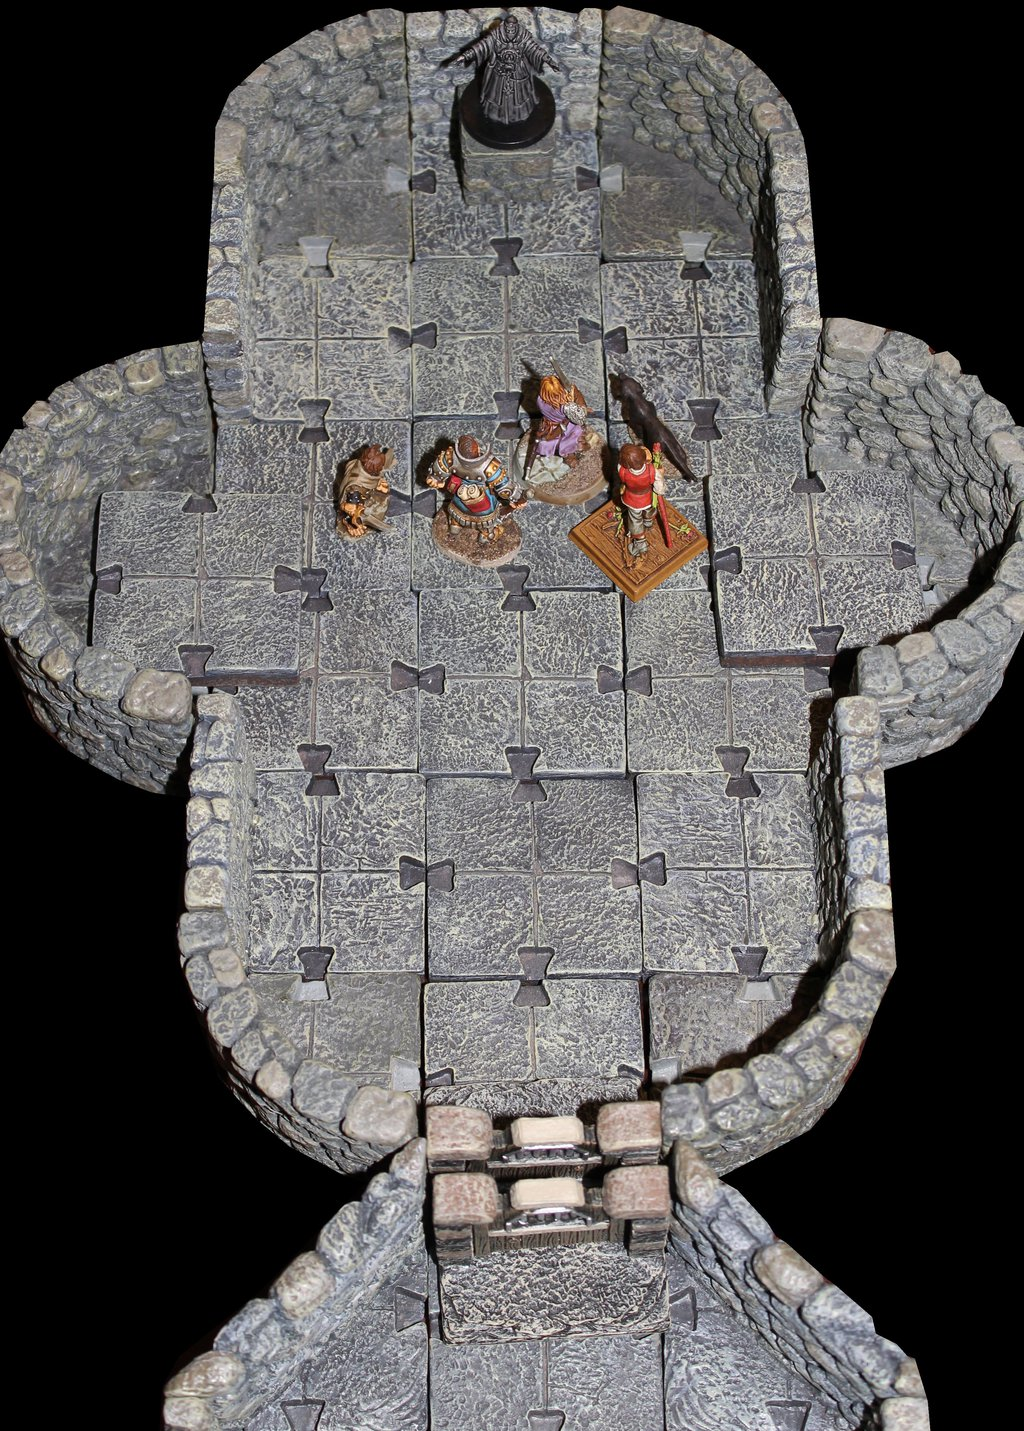
\includegraphics[width=0.39\textwidth]{images/Vivified-labyrinth-entrance-563930398.jpg}
	\caption{Vivified labyrinth entrance}
	\label{fig:Vivified-labyrinth-entrance-563930398}
\end{figure}

Behind this is a large room which is filled with a pool of acid. A stone walkway leads to a central platform with a shining circular symbol in the middle.\hyperref[fig:Vivified-labyrinth-air-elemental-over-acid-pit-563931191]{ As Sjo steps on the platform, the circle flashes up even brighter and summons a huge air elemental which immediately slams down on the Shoanti. } Puk gets hit as well as he tries to tumble into position, but the halfling quickly discovers that the creature is invulnerable to his vicious sneak attacks. Balian jumps into the fray as well, but needs Quint's  {\itshape timely inspiration} to actually hit the swirling air. The bard follows up with a  {\itshape haste} spell. Sjo calls upon his fiery wings and flies to the other end of the platform, catching the agile creature in his  {\itshape burning hands} flames, but causing it hardly any harm. The combatants exchange some hits and slams while first Spyder, next Puk and then Quint get sucked up in the whirlwind and spat out in the pool of acid. Fortunately Balian and Sjo get the better of the air elemental and quickly pull their allies out of the biting fluid. \\

\begin{figure}[h]
	\centering
	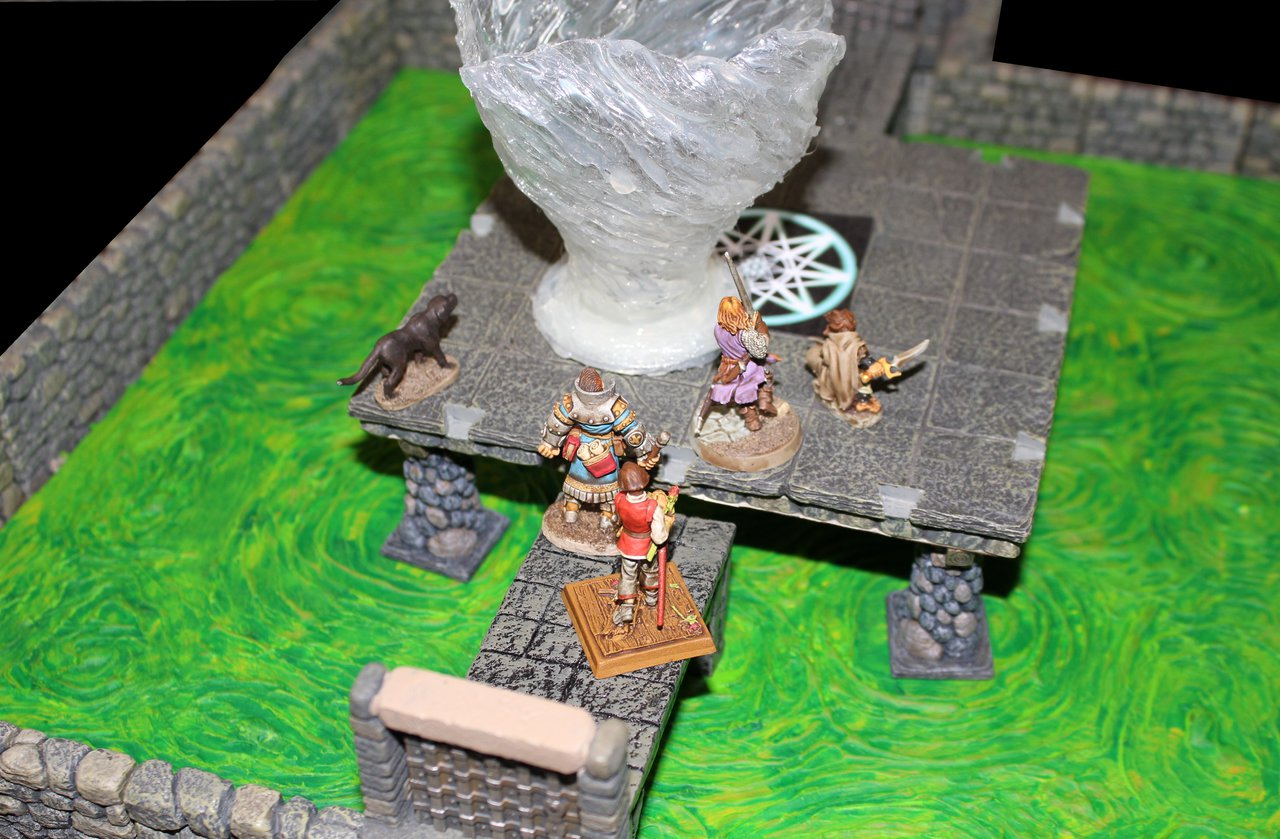
\includegraphics[width=0.39\textwidth]{images/Vivified-labyrinth-air-elemental-over-acid-pit-563931191.jpg}
	\caption{Vivified labyrinth air elemental over acid pit}
	\label{fig:Vivified-labyrinth-air-elemental-over-acid-pit-563931191}
\end{figure}

Behind the acid pool is another corridor with a corner in the beginning.\hyperref[fig:Vivified-labyrinth-gold-mirror-puzzle-563931764]{ A gold mirror is mounted on the wall. } Words have been written into the frame: "Use me, but do not speak about me or I will break." Discussing this strange puzzle, Quint uses the word 'mirror' several times, but that has no (ill) effect whatsoever. Balian finds that trying to take the mirror off the wall is not possible. Sjo notices a strong aura of conjuration magic down the corridor and tries to study the corridor in the reflection of the mirror, but cannot figure out how this puzzle works. Puk and Balian find no traps of pressure plates, but when they throw a gold piece down the hall, it reappears in the corner. So the corridor teleports you back, unless you use whatever it is you have to use. \\

\begin{figure}[h]
	\centering
	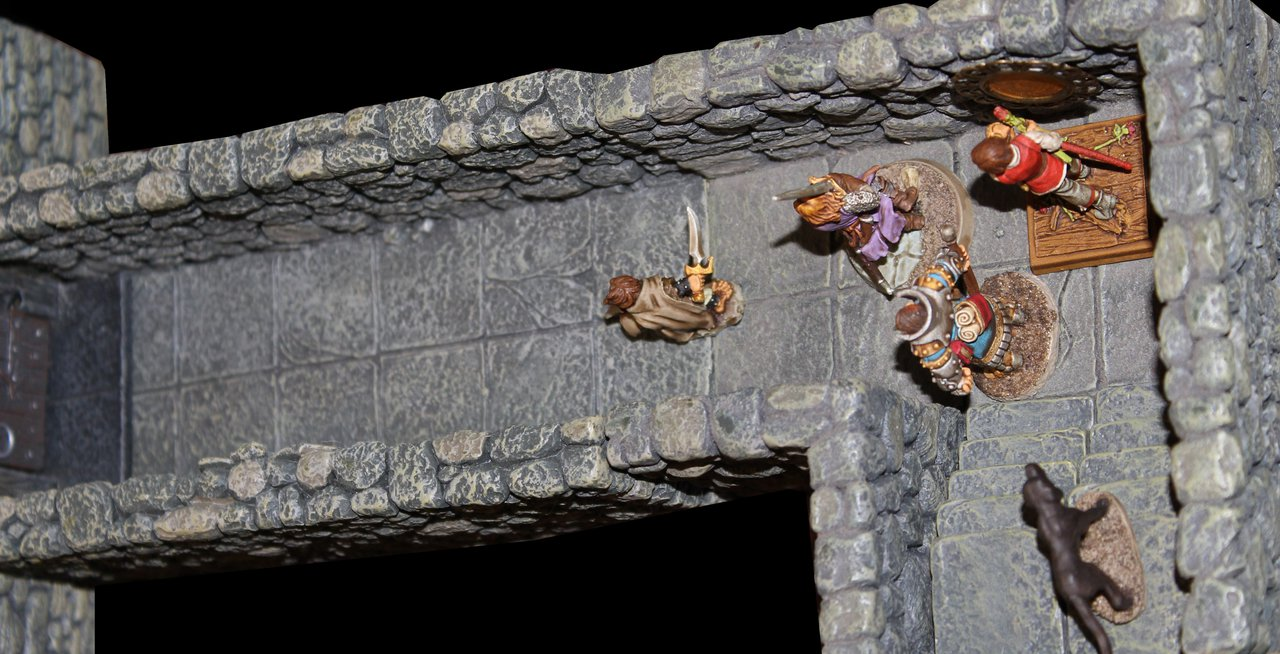
\includegraphics[width=0.39\textwidth]{images/Vivified-labyrinth-gold-mirror-puzzle-563931764.jpg}
	\caption{Vivified labyrinth gold mirror puzzle}
	\label{fig:Vivified-labyrinth-gold-mirror-puzzle-563931764}
\end{figure}

Suddenly Puk steps up, looking at the mirror, and says: "It a riddle. What can break when you say it?"\\

"A secret is gone when you speak it out loud," Quint muses, "but how do you {\itshape use} a secret here? And what has this mirror to do with it?" Meanwhile Sjo attempts to walk down the hallway, but also gets teleported back to the beginning. "It might not be the mirror, but the fact that it is made of gold that is the hint", Puk tries. "What is gold? The sun? The rays of the sun? Should we summon light or something?"\\

"Silence ..." Quint thinks out loud. "Silence is golden. And when you utter the word, you break the silence. You have to be silent to walk to the other side."\\

"I'll give it a try", Puk says as he tiptoes to the far end of the corridor. This time he is not teleported back, but he reaches the door on the other side. Opening it, the halfling stares into a small room with bookcases lining the side walls and many books and scrolls spread out on the floor. Now that the door is open, Puk's friends can easily join him, but when they step into the library,\hyperref[fig:Scrivenite-in-the-vivified-labyrinth-563932189]{ the books float off the ground and swirl together to form a creature made of tomes and scrolls } . \\

\begin{figure}[h]
	\centering
	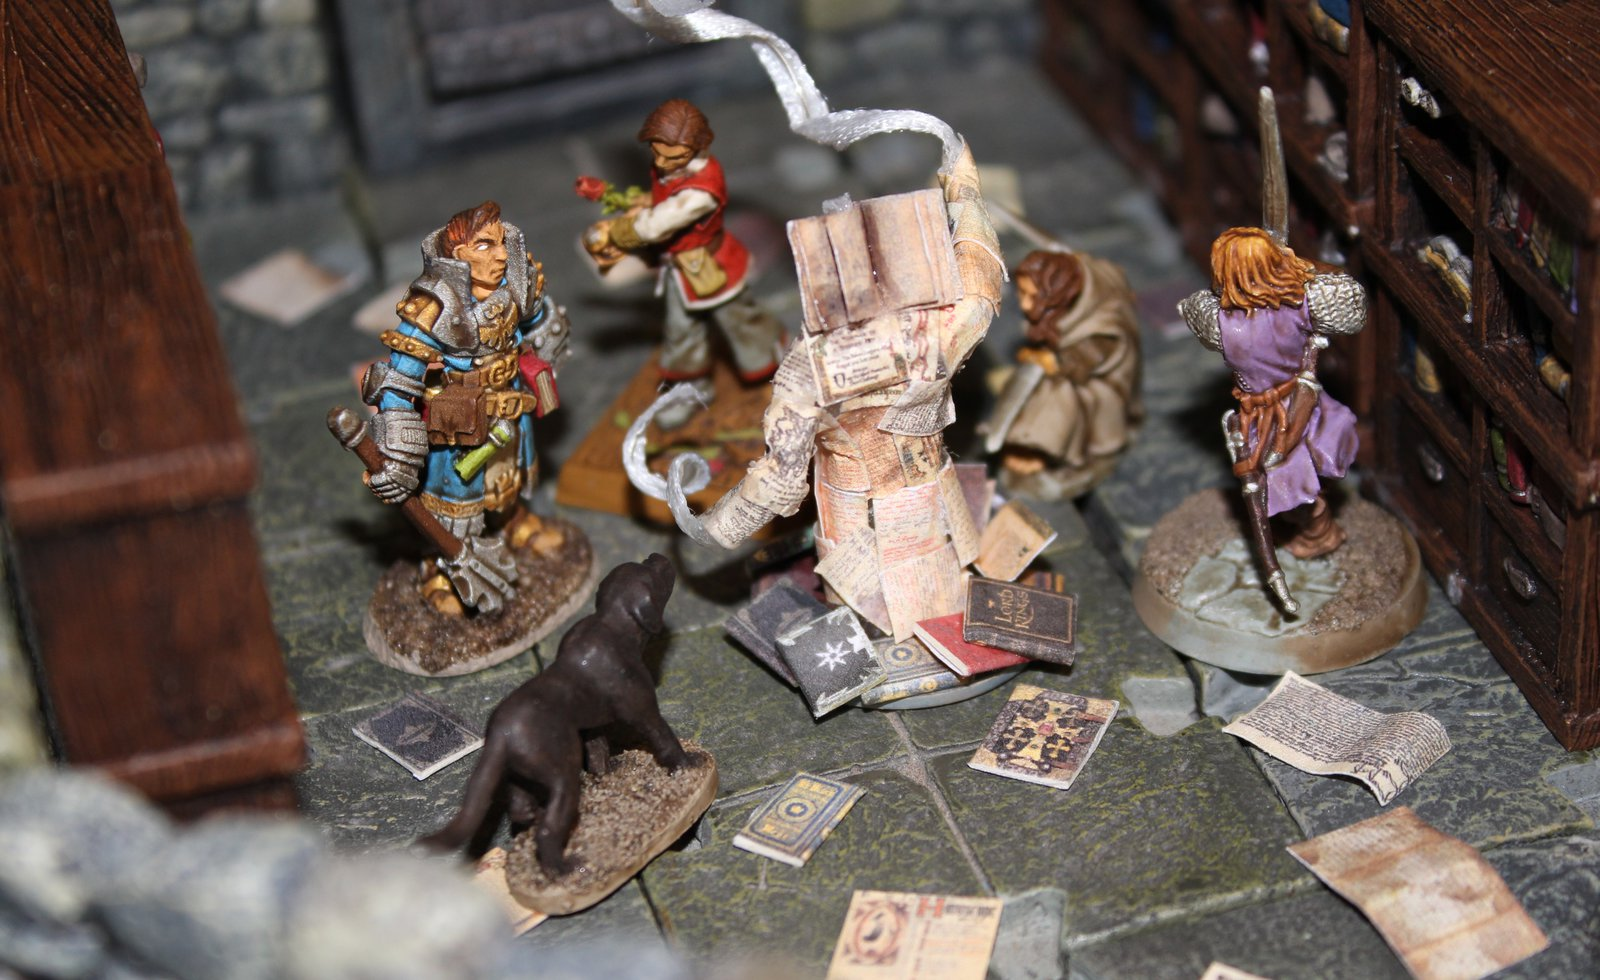
\includegraphics[width=0.39\textwidth]{images/Scrivenite-in-the-vivified-labyrinth-563932189.jpg}
	\caption{Scrivenite in the vivified labyrinth}
	\label{fig:Scrivenite-in-the-vivified-labyrinth-563932189}
\end{figure}

